\documentclass[12pt,a4paper]{article}
\usepackage[a4paper,margin=2.6cm]{geometry}
\usepackage[T1]{fontenc}
\usepackage[sc]{mathpazo}          % Palatino text + matching maths: heavier and easier to read than Computer Modern
\usepackage[scaled=0.92]{helvet}   % sans-serif headings
\linespread{1.18}
\usepackage[parfill]{parskip}
\usepackage{amsmath,amssymb,bm}
\usepackage{graphicx,booktabs,array}
\usepackage[dvipsnames]{xcolor}
\usepackage{tikz}
\usetikzlibrary{arrows.meta,calc}
\usepackage[most]{tcolorbox}
\usepackage{enumitem}
\setlist{itemsep=3pt,topsep=4pt}
\usepackage[font=small,labelfont=bf,margin=0.5cm]{caption}
\usepackage{titlesec}
\titleformat{\section}{\sffamily\Large\bfseries\color{MidnightBlue}}{\thesection}{0.6em}{}
\titleformat{\subsection}{\sffamily\large\bfseries}{\thesubsection}{0.6em}{}
\titlespacing*{\section}{0pt}{20pt}{8pt}
\titlespacing*{\subsection}{0pt}{12pt}{4pt}
\usepackage{fancyhdr}
\pagestyle{fancy}\fancyhf{}
\fancyhead[L]{\sffamily\small Lens + pinhole holography: theory}
\fancyhead[R]{\sffamily\small\thepage}
\renewcommand{\headrulewidth}{0.3pt}\setlength{\headheight}{15pt}
\usepackage[colorlinks=true,linkcolor=MidnightBlue,urlcolor=MidnightBlue,citecolor=MidnightBlue]{hyperref}

% boxes
\newtcolorbox{short}{colback=MidnightBlue!5,colframe=MidnightBlue!70,boxrule=0.6pt,arc=3pt,left=8pt,right=8pt,top=6pt,bottom=6pt,
  title=In short,fonttitle=\sffamily\bfseries}
\newtcolorbox{tool}{colback=ForestGreen!5,colframe=ForestGreen!70!black,boxrule=0.6pt,arc=3pt,left=8pt,right=8pt,top=6pt,bottom=6pt,
  title=In the simulator,fonttitle=\sffamily\bfseries}
\newtcolorbox{limit}{colback=orange!6,colframe=orange!70!black,boxrule=0.6pt,arc=3pt,left=8pt,right=8pt,top=6pt,bottom=6pt,
  title=Limitation of the model,fonttitle=\sffamily\bfseries}
\newtcolorbox{keyeq}{colback=gray!5,colframe=gray!50,boxrule=0.5pt,arc=3pt,left=6pt,right=6pt,top=2pt,bottom=2pt}

\newcommand{\F}{\mathcal{F}}
\newcommand{\Prop}{\mathcal{P}}
\newcommand{\ui}{\mathrm{i}}
\newcommand{\dd}{\,\mathrm{d}}
\newcommand{\um}{\,\mu\mathrm{m}}
\newcommand{\mm}{\,\mathrm{mm}}

\begin{document}

\begin{titlepage}
\vspace*{3cm}
{\sffamily\bfseries\Huge\color{MidnightBlue} Lensless Holography Bench\par}
\vspace{6pt}
{\sffamily\Large Theory of the lens + pinhole configuration\par}
\vspace{1.2cm}
\begin{minipage}{0.86\linewidth}
\large
This document explains, step by step and with all equations, what the simulator computes when a
\textbf{focusing lens} concentrates the laser beam onto a \textbf{pinhole}, and the light leaving the
pinhole illuminates the sample and the camera.

Other configurations of the tool (no lens, no pinhole, fibre source, plane-wave illumination) are
deliberately left out.

Every chapter starts with a short plain-language summary, then gives the equations, and ends with the
control in the simulator that sets each quantity. Chapter~\ref{sec:example} works through the complete
chain with the numbers of the default setup, so every equation can be checked against the values the
simulator displays.
\end{minipage}
\vfill
{\sffamily Documentation for the Lensless Holography Bench (CPU and WebGPU versions), October 2026\par}
\end{titlepage}

\tableofcontents
\newpage

%==================================================================
\section{The setup}
\label{sec:setup}

\begin{figure}[h]
\centering
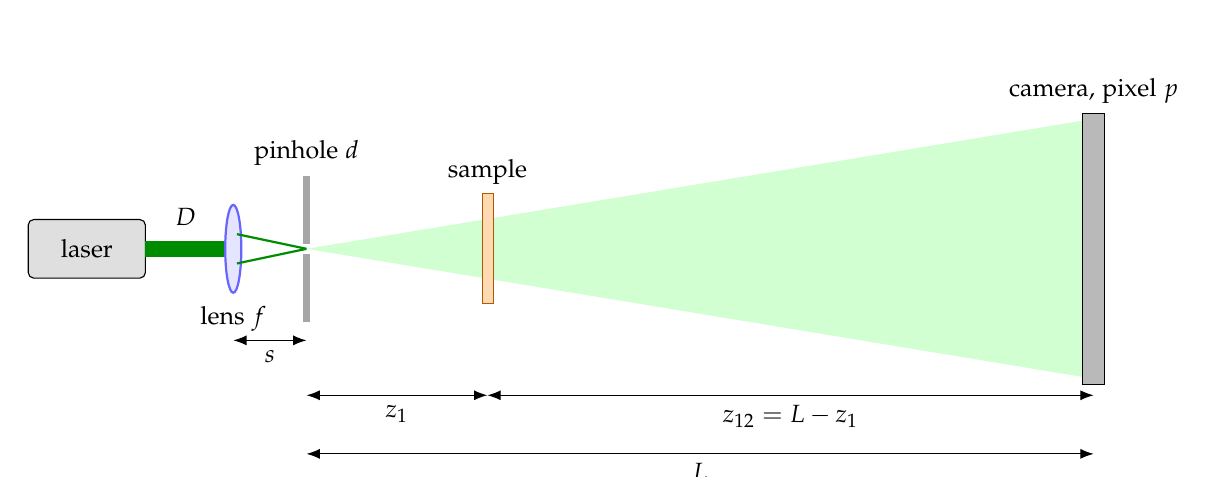
\begin{tikzpicture}[scale=0.93,>=Latex,font=\small]
 % cone
 \fill[green!18] (2.6,0) -- (13.2,1.75) -- (13.2,-1.75) -- cycle;
 % laser
 \draw[fill=gray!25,rounded corners=2pt] (-1.2,-0.4) rectangle (0.4,0.4); \node at (-0.4,0) {laser};
 \draw[green!55!black,line width=6pt] (0.4,0) -- (1.5,0);
 \node[above] at (0.95,0.18) {$D$};
 % lens
 \draw[fill=blue!10,draw=blue!60,thick] (1.6,0) ellipse (0.11 and 0.6); \node[below] at (1.6,-0.65) {lens $f$};
 \draw[green!55!black,thick] (1.65,0.2) -- (2.6,0) (1.65,-0.2) -- (2.6,0);
 % pinhole
 \draw[line width=2.5pt,gray!70] (2.6,0.07) -- (2.6,1.0) (2.6,-0.07) -- (2.6,-1.0); \node[above] at (2.6,1.0) {pinhole $d$};
 % sample
 \draw[fill=orange!30,draw=orange!70!black] (5.0,-0.75) rectangle (5.15,0.75); \node[above] at (5.07,0.75) {sample};
 % camera
 \draw[fill=gray!55] (13.2,-1.85) rectangle (13.5,1.85); \node[above] at (13.35,1.85) {camera, pixel $p$};
 % dims
 \draw[<->] (1.6,-1.25) -- node[below]{$s$} (2.6,-1.25);
 \draw[<->] (2.6,-2.0) -- node[below]{$z_1$} (5.07,-2.0);
 \draw[<->] (5.07,-2.0) -- node[below]{$z_{12}=L-z_1$} (13.35,-2.0);
 \draw[<->] (2.6,-2.8) -- node[below]{$L$} (13.35,-2.8);
\end{tikzpicture}
\caption{The configuration treated in this document. The laser beam (diameter $D$) is focused by a lens of focal length $f$; a pinhole of diameter $d$ sits at distance $s$ behind the lens (normally $s=f$, in the focus). The light diverging from the pinhole illuminates the sample at distance $z_1$; the camera is at distance $L$ from the pinhole. There is no lens between the sample and the camera.}
\label{fig:geom}
\end{figure}

\begin{short}
The lens squeezes the laser beam into a spot of about one micrometre. The pinhole in that spot
removes everything that is not a clean, round spot. What leaves the pinhole is a nearly ideal
\emph{point source}: a smooth spherical wave. The sample sits close to this point source and far from the camera, so its shadow (the hologram) is strongly
magnified on the camera. A computer then turns the hologram back into an image of the sample.
\end{short}

\begin{table}[h]
\centering
\renewcommand{\arraystretch}{1.25}
\begin{tabular}{@{}l >{\raggedright\arraybackslash}p{6.2cm} >{\raggedright\arraybackslash}p{4.4cm}@{}}
\toprule
\textbf{Symbol} & \textbf{Meaning} & \textbf{Control in the tool}\\
\midrule
$\lambda$, $k=2\pi/\lambda$ & wavelength, wavenumber & Laser\\
$D$, $w=D/2$ & laser beam diameter and radius ($1/e^2$) & Laser beam Ø\\
$f$ & focal length of the lens & Lens focal length\\
$\mathrm{NA_L}$ & largest numerical aperture the lens accepts & Lens NA\\
$s$, $\Delta=s-f$ & lens--pinhole distance; offset of the pinhole from the focus & Lens $\to$ pinhole $s$\\
$d$ & pinhole diameter & Pinhole Ø\\
$z_1$ & pinhole--sample distance & Pinhole $\to$ sample $z_1$\\
$L$, $z_{12}$ & pinhole--camera and sample--camera distance & Pinhole $\to$ camera $L$\\
$p$, $N$ & camera pixel pitch; grid size ($N\times N$ points) & Pixel pitch; Sensor\\
$t(x,y)$ & complex transmission of the sample & Sample\\
\bottomrule
\end{tabular}
\caption{Symbols used throughout. All lengths in the simulator are in micrometres unless stated otherwise.}
\end{table}

\subsection*{What the simulator does, in order}
\begin{enumerate}[label=\textbf{\arabic*.}]
\item \textbf{Focus} the laser beam with the lens (Chapter~\ref{sec:focus}).
\item \textbf{Clip} the focus with the pinhole (Chapter~\ref{sec:pinhole}).
\item \textbf{Propagate} the light from the pinhole to the sample, giving the illumination $A(x,y)$ (Chapter~\ref{sec:illum}); add dust on the optics, which the pinhole partly filters out (Chapter~\ref{sec:filter}).
\item \textbf{Multiply} by the sample transmission $t$ and propagate to the camera, using the magnification trick of Chapter~\ref{sec:scaling} and the propagation method of Chapter~\ref{sec:asm}.
\item \textbf{Record} the intensity with a realistic camera (Chapter~\ref{sec:camera}).
\item \textbf{Reconstruct}: propagate back and remove the twin image (Chapter~\ref{sec:recon}).
\item \textbf{Report} resolution, field of view and other numbers (Chapter~\ref{sec:merit}).
\end{enumerate}

%==================================================================
\section{Focusing the laser beam}
\label{sec:focus}

\begin{short}
A wider beam or a shorter focal length gives a larger cone of light and a smaller focal spot.
The lens can only accept a cone up to its own NA; if the beam is wider than that, the lens
aperture clips it.
\end{short}

\subsection{Working numerical aperture}
The beam of radius $w$ arrives collimated at the lens. The half-angle of the cone it forms behind the lens is set by the beam itself, $\mathrm{NA_g}=w/f$, unless the lens aperture is smaller:
\begin{keyeq}
\begin{equation}
\mathrm{NA_g}=\frac{w}{f},\qquad
\mathrm{NA_w}=\min\big(\mathrm{NA_g},\,\mathrm{NA_L}\big).
\label{eq:na}
\end{equation}
\end{keyeq}
If $\mathrm{NA_g}\ge\mathrm{NA_L}$ the lens is \emph{overfilled}. Only the part of the Gaussian beam inside the lens aperture radius $\mathrm{NA_L}f$ is transmitted:
\begin{equation}
T_\mathrm{lens}=1-\exp\!\left[-2\left(\frac{\mathrm{NA_L}\,f}{w}\right)^{2}\right].
\end{equation}

\begin{figure}[h]
\centering
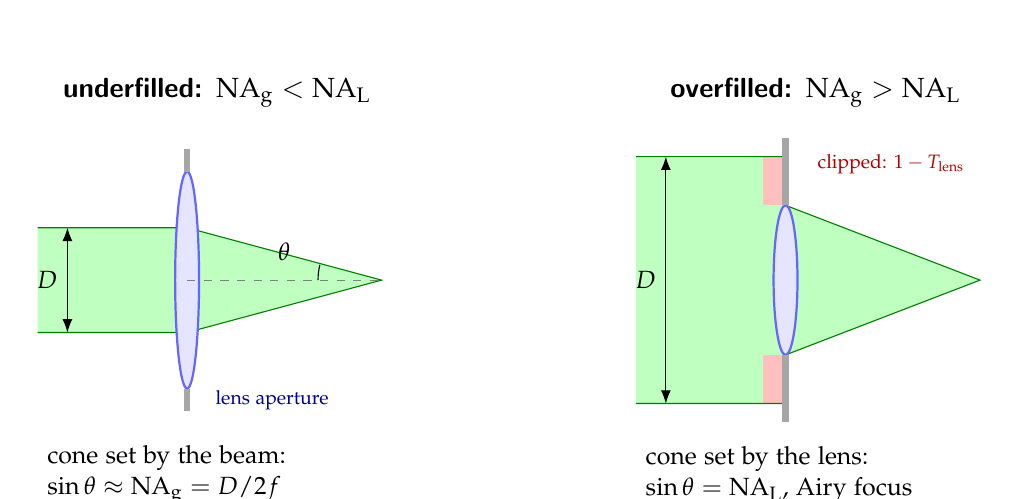
\begin{tikzpicture}[>=Latex,font=\small,scale=0.95]
 % ---- underfilled
 \begin{scope}
  \node[font=\sffamily\bfseries] at (2.4,2.5) {underfilled: $\mathrm{NA_g}<\mathrm{NA_L}$};
  \fill[green!25] (0,0.7) -- (2.0,0.7) -- (4.6,0) -- (2.0,-0.7) -- (0,-0.7) -- cycle;
  \draw[green!50!black] (0,0.7) -- (2.0,0.7) -- (4.6,0) -- (2.0,-0.7) -- (0,-0.7);
  \draw[fill=blue!10,draw=blue!60,thick] (2.0,0) ellipse (0.16 and 1.45);
  \draw[line width=2.4pt,gray!70] (2.0,1.45) -- (2.0,1.75) (2.0,-1.45) -- (2.0,-1.75);
  \draw[<->] (0.4,-0.7) -- node[left]{$D$} (0.4,0.7);
  \draw[dashed,gray] (2.0,0) -- (4.6,0);
  \draw (3.75,0) arc (180:166:0.85); \node at (3.3,0.38) {$\theta$};
  \node[blue!60!black,anchor=west] at (2.25,-1.6) {\scriptsize lens aperture};
  \node[align=left,anchor=west] at (0,-2.6) {cone set by the beam:\\ $\sin\theta\approx\mathrm{NA_g}=D/2f$};
 \end{scope}
 % ---- overfilled
 \begin{scope}[xshift=8.0cm]
  \node[font=\sffamily\bfseries] at (2.4,2.5) {overfilled: $\mathrm{NA_g}>\mathrm{NA_L}$};
  \fill[green!25] (0,1.65) -- (2.0,1.65) -- (2.0,-1.65) -- (0,-1.65) -- cycle;
  \fill[green!25] (2.0,1.0) -- (4.6,0) -- (2.0,-1.0) -- cycle;
  \fill[red!25] (1.7,1.0) rectangle (2.0,1.65); \fill[red!25] (1.7,-1.0) rectangle (2.0,-1.65);
  \draw[green!50!black] (0,1.65) -- (2.0,1.65) (0,-1.65) -- (2.0,-1.65) (2.0,1.0) -- (4.6,0) -- (2.0,-1.0);
  \draw[fill=blue!10,draw=blue!60,thick] (2.0,0) ellipse (0.16 and 1.0);
  \draw[line width=2.4pt,gray!70] (2.0,1.0) -- (2.0,1.9) (2.0,-1.0) -- (2.0,-1.9);
  \draw[<->] (0.4,-1.65) -- node[left]{$D$} (0.4,1.65);
  \node[red!70!black,anchor=west] at (2.3,1.55) {\scriptsize clipped: $1-T_\mathrm{lens}$};
  \node[align=left,anchor=west] at (0,-2.6) {cone set by the lens:\\ $\sin\theta=\mathrm{NA_L}$, Airy focus};
 \end{scope}
\end{tikzpicture}
\caption{The working numerical aperture, Eq.~\eqref{eq:na}. Left: the beam is narrower than the lens aperture, so the beam diameter fixes the cone and the focus is Gaussian. Right: the beam is wider than the aperture; the outer part (red) is blocked, the cone is fixed by the lens and the focus becomes an Airy pattern.}
\label{fig:fill}
\end{figure}

\subsection{Size of the focal spot}
\begin{keyeq}
\begin{equation}
d_\mathrm{spot}=
\begin{cases}
\dfrac{2\lambda}{\pi\,\mathrm{NA_g}} & \text{underfilled lens: Gaussian spot, $1/e^2$ diameter,}\\[10pt]
\dfrac{1.22\,\lambda}{\mathrm{NA_L}} & \text{overfilled lens: Airy spot, diameter of the first dark ring.}
\end{cases}
\label{eq:spot}
\end{equation}
\end{keyeq}

\begin{figure}[h]
\centering
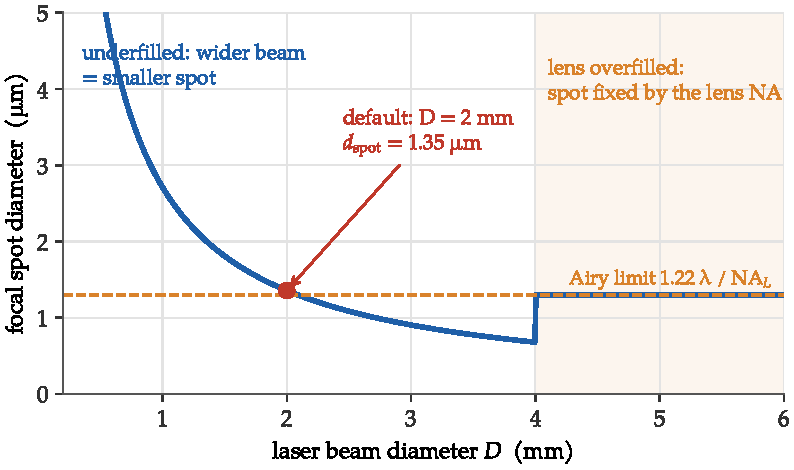
\includegraphics[width=0.86\linewidth]{figs/fig_spot_vs_D.pdf}
\caption{Focal spot diameter from Eq.~\eqref{eq:spot} for $f=4\mm$, $\mathrm{NA_L}=0.5$, $\lambda=532$~nm. Widening the beam shrinks the spot until the lens is overfilled at $D=2\mathrm{NA_L}f=4\mm$; beyond that the lens NA fixes the spot. The jump at 4~mm comes from the model switching between the two formulas. In a real lens the change is gradual, because a partly clipped Gaussian lies between both cases.}
\label{fig:spotD}
\end{figure}

\subsection{The beam near the focus}
Close to the focus the beam is a Gaussian beam. Its waist radius $w_0$, Rayleigh range $z_R$ (the distance over which the spot stays roughly the same size), radius $w(\Delta)$ and wavefront radius of curvature $R(\Delta)$ at a distance $\Delta$ from the focus are
\begin{keyeq}
\begin{equation}
\begin{gathered}
w_0=\frac{\lambda}{\pi\,\mathrm{NA_w}},\qquad
z_R=\frac{\pi w_0^{2}}{\lambda},\\[4pt]
w(\Delta)=w_0\sqrt{1+\left(\frac{\Delta}{z_R}\right)^{2}},\qquad
R(\Delta)=\Delta\left[1+\left(\frac{z_R}{\Delta}\right)^{2}\right].
\end{gathered}
\label{eq:gauss}
\end{equation}
\end{keyeq}
Here $\Delta=s-f$. For $\Delta>0$ the pinhole is behind the focus and the beam is already diverging there ($R>0$); for $\Delta<0$ it is still converging.

\begin{figure}[h]
\centering
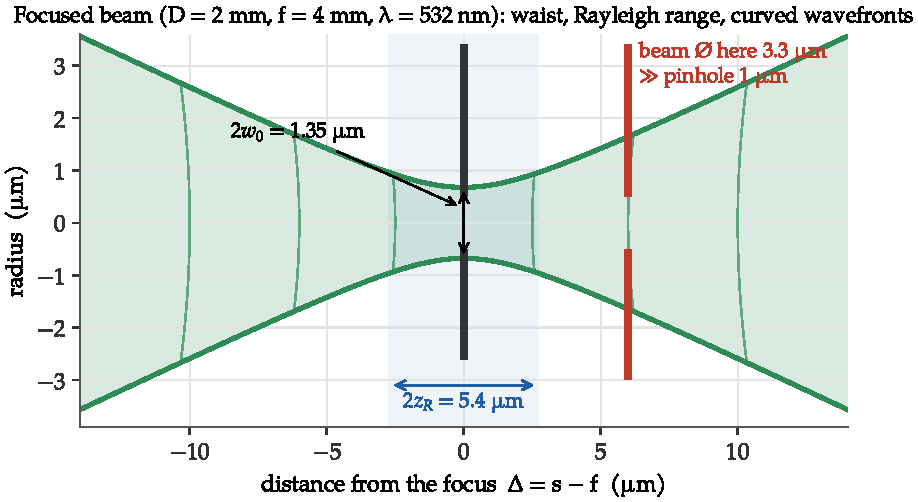
\includegraphics[width=0.92\linewidth]{figs/fig_gauss_focus.pdf}
\caption{The beam near the focus for the default setup, from Eq.~\eqref{eq:gauss}. The waist is $2w_0=1.35\um$ and the beam keeps this size only over $2z_R=5.4\um$ (blue band). Thin lines are wavefronts: flat in the focus, curved on either side. The black pinhole (1~µm) sits in the focus. The red one, only 6~µm further, sees a 3.3~µm beam and passes just 17\,\% of the light (Fig.~\ref{fig:tpin}).}
\label{fig:gauss}
\end{figure}

\begin{tool}
\textbf{Focus on the pinhole} sets $s=f$ ($\Delta=0$). The buttons $\pm1\um$ and $\pm10\um$ move the pinhole along the axis.
``Focus'' shows $d_\mathrm{spot}$ and $\mathrm{NA_w}$; ``Beam at pinhole'' shows $2w(\Delta)$, $\Delta$ and $z_R$.
\end{tool}

Because $z_R$ is only a few micrometres for a tightly focused beam, a focus error of a few micrometres already makes the beam at the pinhole much wider than the waist. This is why the pinhole position must be adjusted so finely in a real spatial filter (Fig.~\ref{fig:gauss}).

%==================================================================
\section{The pinhole}
\label{sec:pinhole}

\begin{short}
The pinhole passes the central spot and blocks light that arrives at an angle, which is mostly
light scattered by dust and lens imperfections. If the pinhole is too small it also cuts into the
spot and wastes power. If it is too large it filters nothing.
\end{short}

\begin{figure}[h]
\centering
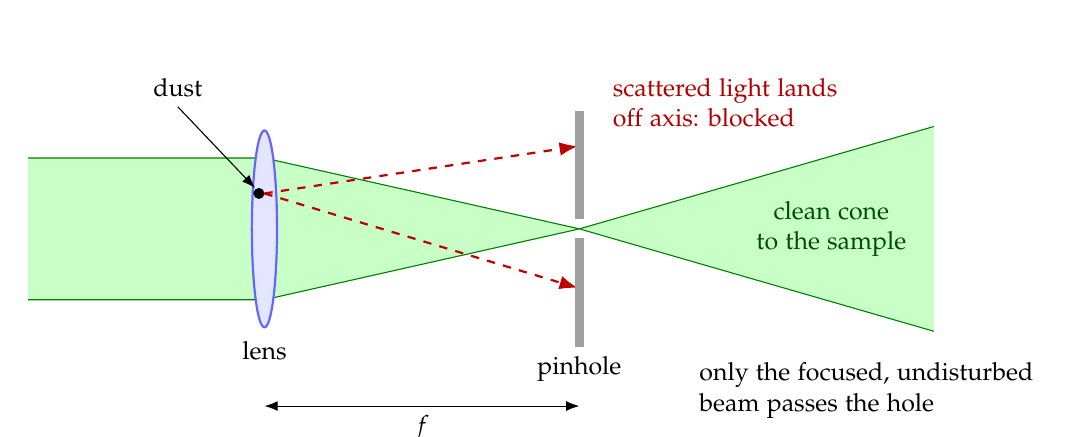
\begin{tikzpicture}[>=Latex,font=\small]
 \fill[green!22] (0,0.9) -- (3,0.9) -- (7,0) -- (3,-0.9) -- (0,-0.9) -- cycle;
 \fill[green!22] (7,0) -- (11.5,1.3) -- (11.5,-1.3) -- cycle;
 \draw[green!50!black] (0,0.9) -- (3,0.9) -- (7,0) -- (11.5,1.3) (0,-0.9) -- (3,-0.9) -- (7,0) -- (11.5,-1.3);
 \draw[fill=blue!10,draw=blue!60,thick] (3,0) ellipse (0.16 and 1.25); \node[below] at (3,-1.3) {lens};
 \fill[black] (2.93,0.45) circle (0.07); \draw[->] (1.9,1.55) node[above]{dust} -- (2.88,0.52);
 % scattered light from the dust: tilted rays meeting the focal plane off axis
 \draw[red!75!black,thick,dashed,->] (3.0,0.45) -- (6.98,1.05);
 \draw[red!75!black,thick,dashed,->] (3.0,0.45) -- (6.98,-0.75);
 \draw[line width=3pt,gray!75] (7,0.12) -- (7,1.5) (7,-0.12) -- (7,-1.5);
 \node[below] at (7,-1.5) {pinhole};
 \node[red!70!black,align=left,anchor=west] at (7.3,1.6) {scattered light lands\\off axis: blocked};
 \draw[<->] (3,-2.25) -- node[below]{$f$} (7,-2.25);
 \node[green!30!black,align=center] at (10.2,0) {clean cone\\ to the sample};
 \node[align=left,anchor=west] at (8.4,-2.05) {only the focused, undisturbed\\beam passes the hole};
\end{tikzpicture}
\caption{Why the pinhole cleans the beam. The lens sends each \emph{direction} of light to a different \emph{point} in its focal plane. The clean, parallel beam goes to the centre and passes the hole. Light scattered by dust or scratches travels at other angles, so it reaches the focal plane off axis and is stopped. Chapter~\ref{sec:filter} turns this into a low-pass filter with cut-off $\nu_c=d/(2\lambda|z_s|)$.}
\label{fig:filter}
\end{figure}

\subsection{Transmitted power}
For a Gaussian of local radius $w_g=w(\Delta)$ centred on a circular hole of diameter $d$,
\begin{keyeq}
\begin{equation}
T_\mathrm{pin}=1-\exp\!\left(-\frac{2\,(d/2)^{2}}{w_g^{2}}\right),
\qquad T=T_\mathrm{lens}\,T_\mathrm{pin}.
\label{eq:tpin}
\end{equation}
\end{keyeq}
For an overfilled lens with the pinhole exactly in focus the spot is an Airy pattern, and the simulator uses $T_\mathrm{pin}\approx\min[1,(d/d_\mathrm{spot})^2]$.

\paragraph{Practical rule.} A pinhole of $d\approx1.5\,d_\mathrm{spot}$ (that is $d/2=1.5\,w_0$) transmits $1-e^{-4.5}\approx99\,\%$ of a Gaussian focus while still blocking light that arrives more than a few spot radii off axis. Smaller pinholes give a cleaner, more point-like source but lose power; see the example in Chapter~\ref{sec:example}.

\begin{figure}[h]
\centering
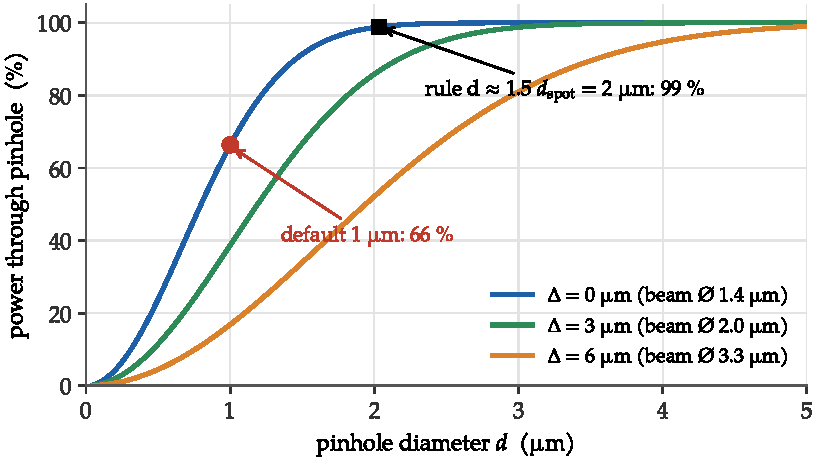
\includegraphics[width=0.86\linewidth]{figs/fig_Tpin.pdf}
\caption{Power through the pinhole, Eq.~\eqref{eq:tpin}, for the default focus ($2w_0=1.35\um$). Blue: pinhole in focus. Green and orange: pinhole 3 and 6~µm out of focus, where the beam is wider. The red dot is the default 1~µm pinhole (66\,\%), the black square the 1.5\,$d_\mathrm{spot}$ rule (99\,\%).}
\label{fig:tpin}
\end{figure}

\subsection{Three regimes}
The simulator compares the pinhole with the beam through the ratio
\begin{equation}
\mathrm{ratio}=\frac{d}{2\,w_g}
\end{equation}
and names the regime under ``Illumination'':
\begin{center}
\renewcommand{\arraystretch}{1.3}
\begin{tabular}{@{}p{3.0cm} p{3.2cm} p{8.0cm}@{}}
\toprule
\textbf{Regime} & \textbf{Condition} & \textbf{What leaves the pinhole}\\
\midrule
point source & ratio $<0.5$ (and flat wavefront) & a small, almost uniformly lit hole: an Airy cone\\
clipped beam & $0.5\le$ ratio $\le2$ & the edge of the Gaussian is cut: a mixture of both\\
focused spot & ratio $>2$ & the pinhole hardly touches the beam: a Gaussian cone from the focus\\
\bottomrule
\end{tabular}
\end{center}

\begin{figure}[h]
\centering
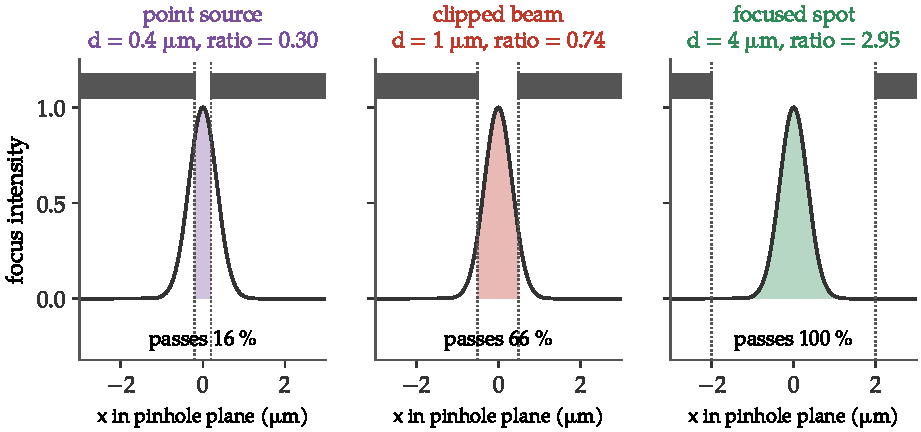
\includegraphics[width=\linewidth]{figs/fig_regimes.pdf}
\caption{The three regimes, drawn to scale for the default focus. The black curve is the intensity of the focal spot, the grey bars are the pinhole plate, and the coloured area is the light that passes. Left: the hole samples only the flat top of the spot, so it acts like a tiny, evenly lit hole. Middle: the hole cuts the edges of the spot. Right: the hole is much wider than the spot and does not touch it.}
\label{fig:regimes}
\end{figure}

\subsection{Cone angle}
The half-angle of the illumination cone is
\begin{equation}
\theta=\begin{cases}
\theta_\mathrm{Airy}=\arcsin\dfrac{1.22\,\lambda}{d} & \text{point source,}\\[8pt]
\theta_\mathrm{beam}=\arcsin\mathrm{NA_w} & \text{focused spot,}\\[4pt]
\max(\theta_\mathrm{Airy},\theta_\mathrm{beam}) & \text{clipped beam.}
\end{cases}
\label{eq:cone}
\end{equation}
If the pinhole is far from the focus ($|\Delta|$ large), the cone is further limited by the geometric shadow of the hole, $\arctan[(d/2)/|\Delta|]$.

\begin{figure}[h]
\centering
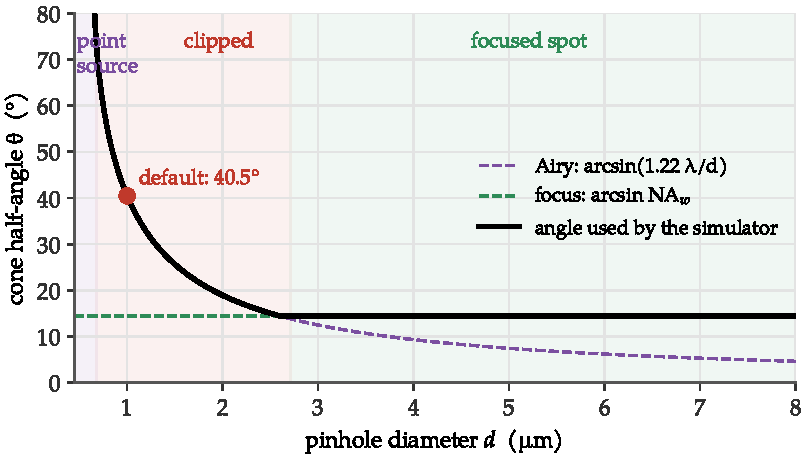
\includegraphics[width=0.86\linewidth]{figs/fig_cone.pdf}
\caption{Cone half-angle, Eq.~\eqref{eq:cone}, against pinhole diameter for the default focus. Small pinholes diffract strongly (Airy, purple dashed line). Large pinholes pass the cone of the lens unchanged (green dashed line, $\arcsin0.25=14.5^\circ$). The black line is what the simulator uses; the background colours mark the three regimes.}
\label{fig:cone}
\end{figure}

%==================================================================
\section{Illumination at the sample}
\label{sec:illum}

\begin{short}
The simulator computes the light pattern on the sample from the field in the pinhole with one
diffraction integral. A small pinhole gives the familiar Airy disk pattern. A large one gives the
smooth Gaussian cone of the focus. Everything in between comes out of the same formula.
\end{short}

\begin{figure}[h]
\centering
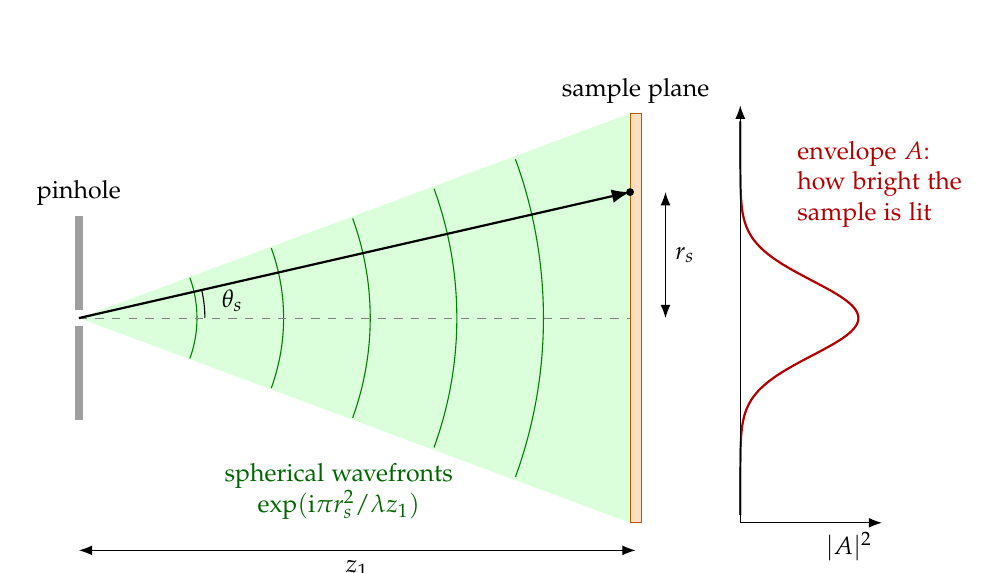
\begin{tikzpicture}[>=Latex,font=\small]
 \fill[green!14] (0,0) -- (7.0,2.6) -- (7.0,-2.6) -- cycle;
 \draw[line width=3pt,gray!75] (0,0.1) -- (0,1.3) (0,-0.1) -- (0,-1.3); \node[above] at (0,1.3) {pinhole};
 \foreach \R in {1.5,2.6,3.7,4.8,5.9} { \draw[green!50!black,thin] ({\R*cos(20)},{\R*sin(20)}) arc (20:-20:\R); }
 \draw[fill=orange!25,draw=orange!70!black] (7.0,-2.6) rectangle (7.15,2.6); \node[above] at (7.07,2.6) {sample plane};
 \draw[dashed,gray] (0,0) -- (7.0,0);
 \draw[->,thick] (0,0) -- (7.0,1.6); \fill (7.0,1.6) circle (0.05);
 \draw (1.6,0) arc (0:12.9:1.6); \node at (1.95,0.22) {$\theta_s$};
 \draw[<->] (7.45,0) -- node[right]{$r_s$} (7.45,1.6);
 \draw[<->] (0,-2.95) -- node[below]{$z_1$} (7.07,-2.95);
 % envelope |A| drawn against the sample plane
 \draw[thick,red!70!black,domain=-2.5:2.5,samples=80,smooth] plot ({8.4+1.5*exp(-2.2*\x*\x)},\x);
 \draw[->] (8.4,-2.6) -- (8.4,2.7); \draw[->] (8.4,-2.6) -- (10.2,-2.6) node[below left]{$|A|^2$};
 \node[red!70!black,align=left,anchor=west] at (9.0,1.7) {envelope $A$:\\ how bright the\\ sample is lit};
 \node[green!40!black,align=center] at (3.3,-2.2) {spherical wavefronts\\ $\exp(\ui\pi r_s^2/\lambda z_1)$};
\end{tikzpicture}
\caption{How the illumination is described, Eq.~\eqref{eq:Adef}. The pinhole emits spherical waves (green arcs). The simulator separates the field on the sample into the ideal spherical phase and a slowly varying envelope $A$ (red), which carries the brightness, the Airy rings and any clipping. A point at height $r_s$ is seen from the pinhole at the angle $\theta_s$, and $A$ depends only on $\sin\theta_s/\lambda$.}
\label{fig:spherical}
\end{figure}

\subsection{Field in the pinhole}
Just behind the pinhole, inside the opening $r<d/2$, the field is the Gaussian beam with its curvature:
\begin{equation}
U_\mathrm{pin}(r)=g(r)\,\exp\!\left(\frac{\ui\pi r^2}{\lambda R}\right),\qquad g(r)=\exp\!\left(-\frac{r^2}{w_g^2}\right).
\end{equation}

\subsection{Radial diffraction integral}
The field at the sample is a spherical wave from the pinhole centre times a slowly varying envelope $A$:
\begin{equation}
U_\mathrm{ill}(x,y)=A(x,y)\,\exp\!\left(\frac{\ui\pi r_s^2}{\lambda z_1}\right),
\label{eq:Adef}
\end{equation}
where $r_s$ is the distance from the axis in the sample plane. For a round pinhole, the Fresnel diffraction integral reduces to a one-dimensional Hankel transform:
\begin{keyeq}
\begin{equation}
\begin{gathered}
A(\rho)=\int_0^{a} g(r)\,\exp\!\left[\frac{\ui\pi r^2}{\lambda}\left(\frac{1}{z_1}+\frac{1}{R}\right)\right] J_0(2\pi\rho r)\,r\dd r,\\[6pt]
\rho=\frac{\sin\theta_s}{\lambda},\qquad \sin\theta_s=\frac{r_s}{\sqrt{r_s^2+z_1^2}}.
\end{gathered}
\label{eq:hankel}
\end{equation}
\end{keyeq}
$J_0$ is the Bessel function of order zero and $a=\min(d/2,\,4w_g)$; beyond $4w_g$ the Gaussian is negligible. Writing $\rho$ with $\sin\theta_s$ instead of the paraxial $r_s/(\lambda z_1)$ keeps the cone correct at larger angles.

\paragraph{Check: the two limits.}
\begin{itemize}
\item \emph{Pinhole much smaller than the beam} ($g\approx1$, curvature negligible). The integral gives the Airy pattern
\begin{equation}
A\propto\frac{2J_1(u)}{u},\qquad u=\frac{\pi d\sin\theta_s}{\lambda},
\end{equation}
whose first zero is at $\sin\theta_s=1.22\lambda/d$, as in Eq.~\eqref{eq:cone}.
\item \emph{Pinhole much larger than the beam}. The integral becomes the Hankel transform of the full Gaussian: again a Gaussian, the cone of the focus with half-width $\mathrm{NA_w}$.
\end{itemize}

\begin{figure}[h]
\centering
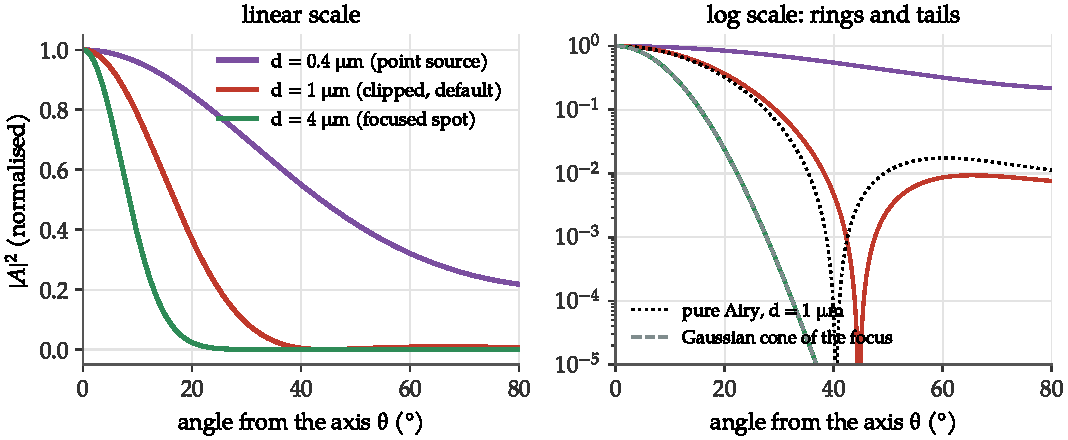
\includegraphics[width=\linewidth]{figs/fig_hankel_profiles.pdf}
\caption{Illumination profiles computed from Eq.~\eqref{eq:hankel} for the default focus with three pinholes. Left: a 0.4~µm hole gives a very wide, nearly flat cone, and a 4~µm hole gives the narrow Gaussian cone of the lens. Right, on a logarithmic scale: the 1~µm curve (red) has the first dark ring of the Airy pattern near $40^\circ$, close to the pure Airy function (dotted). The 4~µm curve follows the Gaussian cone of the focus (dashed grey). Both limits of the integral check out.}
\label{fig:profiles}
\end{figure}

\begin{figure}[h]
\centering
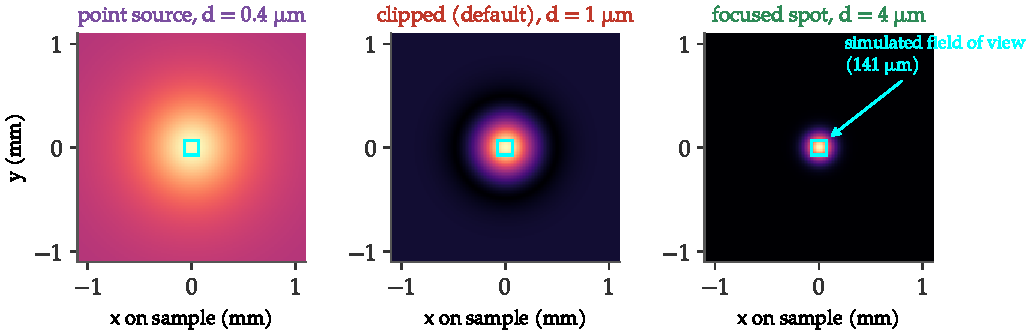
\includegraphics[width=\linewidth]{figs/fig_illum_2d.pdf}
\caption{The same three cases as seen on the sample, $z_1=0.5\mm$ from the pinhole (square root of intensity, for visibility). The cyan square is the 141~µm field of view of the default simulation. Inside it the illumination is almost uniform in all three cases, which is why the default image looks evenly lit even with the clipped 1~µm pinhole.}
\label{fig:illum2d}
\end{figure}

\begin{figure}[h]
\centering
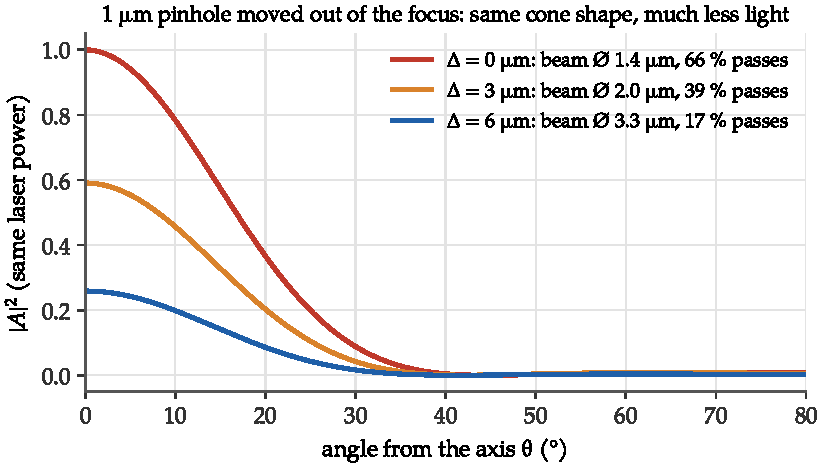
\includegraphics[width=0.86\linewidth]{figs/fig_defocus.pdf}
\caption{Effect of the curvature term $1/R$ in Eq.~\eqref{eq:hankel}: the 1~µm pinhole 0, 3 and 6~µm behind the focus, all at the same laser power. The cone keeps nearly the same shape, because the hole is still smaller than the beam, but most of the light is lost. A misplaced pinhole therefore shows up first as a \emph{dark} hologram (low signal and SNR) rather than as a different pattern.}
\label{fig:defocus}
\end{figure}

\paragraph{Near-field check.} The pinhole Fresnel number
\begin{equation}
N_F=\frac{a_\mathrm{eff}^2}{4\lambda z_1},\qquad a_\mathrm{eff}=\min(d,\,2w_g),
\end{equation}
tells whether the sample is in the far field of the pinhole ($N_F\ll1$, a clean cone) or in its near field ($N_F\gtrsim1$, a ringing image of the hole). With a micrometre-sized pinhole $N_F$ is essentially zero.

\paragraph{Numerics.} Eq.~\eqref{eq:hankel} is evaluated with the midpoint rule. The number of radial samples is chosen so that the phase changes by at most $0.15$~rad per step, with between 300 and 24\,000 samples. $A(\rho)$ is tabulated at 1537 values and interpolated onto the simulation grid.

\subsection{Normalisation}
$A$ is scaled so that its root-mean-square amplitude over the lit area is 1. The lit area is where $|A|^2>0.04\max|A|^2$. Absolute power enters only in the camera model (Chapter~\ref{sec:camera}).

%==================================================================
\section{Why the pinhole helps: spatial filtering}
\label{sec:filter}

\begin{short}
Dust and scratches on the lens throw shadows and fringes into the beam. In the focal plane these
defects show up as light \emph{away} from the central spot. The pinhole blocks that light, so the
illumination at the sample is smooth again. This is the reason a pinhole is used at all.
\end{short}

Behind the focus, the light cone is a magnified image of the lens pupil. A point at radius $r_L$ on the lens maps to
\begin{equation}
r_s=m\,r_L,\qquad m=\frac{|z_s|}{f},\qquad z_s=z_1+\Delta,
\end{equation}
in the sample plane, where $z_s$ is the distance from the focus to the sample.

\subsection{Dirt model}
The simulator places random dust disks on the pupil (radius 10--150~µm, opacity 0.25--0.85; their number grows with the ``Dirt on optics'' setting). It also adds one weak interference fringe from a reflection, of relative amplitude $\epsilon=0.12\times\text{dirt}$:
\begin{equation}
\mathcal{D}(x,y)=\prod_i\big[1-o_i\,\Pi_i(x,y)\big],\qquad
A_\mathrm{real}=A\cdot\mathrm{LP}\Big\{\sqrt{\mathcal{D}}\,\big[1+\epsilon\cos(2\pi\bm\kappa\cdot\bm x)\big]\Big\}.
\end{equation}

\subsection{The pinhole is a low-pass filter}
A spatial frequency $\nu$ (in cycles per micrometre) of the pattern on the sample comes from the point $\xi=\lambda z_s\nu$ in the focal plane. The pinhole lets through only $|\xi|<d/2$, so it removes every frequency above
\begin{keyeq}
\begin{equation}
\nu_c=\frac{d}{2\lambda|z_s|}.
\label{eq:lp}
\end{equation}
\end{keyeq}
Sharp dust shadows consist of high frequencies and are removed; the smooth beam profile passes. A \emph{smaller} pinhole filters more strongly. The dirty field $A_\mathrm{real}$ lights the sample and forms the hologram, but the reconstruction only knows the clean model $A$. Whatever the pinhole fails to remove therefore appears as an artefact in the reconstructed image.

\begin{tool}
Set ``Dirt on optics'' above zero, then compare a 1~µm pinhole with a large one (e.g.\ 20~µm). With the large pinhole the dust shadows reappear in the hologram and in the reconstruction.
\end{tool}

%==================================================================
\section{Magnification: the equivalent plane-wave hologram}
\label{sec:scaling}

\begin{short}
A hologram recorded with a diverging (spherical) wave looks exactly like a plane-wave hologram
that has been magnified by $M=L/z_1$ and recorded at a shorter, ``effective'' distance. This lets
the simulator work on one grid for any magnification.
\end{short}

The Fresnel scaling theorem \cite{Paganin} gives
\begin{keyeq}
\begin{equation}
M=\frac{L}{z_1},\qquad
z_\mathrm{eff}=\frac{z_1\,z_{12}}{L},\qquad
I_\mathrm{cam}(X,Y)=\frac{1}{M^2}\left|\Prop_{z_\mathrm{eff}}\{A\,t\}\left(\frac{X}{M},\frac{Y}{M}\right)\right|^{2},
\label{eq:scaling}
\end{equation}
\end{keyeq}
where $\Prop_z$ is free-space propagation over the distance $z$ (Chapter~\ref{sec:asm}). Each camera pixel therefore corresponds to a sample-plane size of
\begin{equation}
\delta x=\frac{p}{M},\qquad \text{field of view}=N\,\delta x=\frac{N\,p}{M}.
\end{equation}
The simulation grid is placed in the sample plane with this spacing, so grid point $(i,j)$ is exactly camera pixel $(i,j)$.

\paragraph{Effective source position.} If the pinhole is not exactly at the focus and the beam passes it without much clipping, the light really diverges from the focus, a distance $\Delta$ from the pinhole. The magnification then becomes $M_\mathrm{eff}=(L+\Delta)/(z_1+\Delta)$. In the normal case $\Delta=0$ the two are equal.

%==================================================================
\section{The sample}
\label{sec:sample}
The sample is treated as a thin mask, $t(x,y)=a(x,y)\,e^{\ui\phi(x,y)}$, with amplitude $a$ and phase delay
\begin{equation}
\phi=k\,\Delta n\,h,
\end{equation}
for local thickness $h$ and refractive-index difference $\Delta n$ to the surroundings.
\begin{center}
\renewcommand{\arraystretch}{1.25}
\begin{tabular}{@{}p{4.0cm} p{2.6cm} p{7.4cm}@{}}
\toprule
\textbf{Sample} & \textbf{Amplitude} & \textbf{Phase}\\
\midrule
etched glass letters & 1 & $k(n-1)h_\mathrm{etch}$ inside the letters\\
microspheres & 1 & $k(n_b-n_m)\,2\sqrt{R^2-r^2}$\\
red blood cells & 1 & $k(n_c-n_m)\,h(r)$, biconcave profile \cite{Evans}\\
opaque particles & 0 inside & 0\\
chrome bar target & 0 on the bars & 0\\
phase bar target & 1 & $\phi_\mathrm{max}$ on the bars\\
\bottomrule
\end{tabular}
\end{center}
\begin{limit}
Thin-sample approximation: light is not refracted or scattered several times inside the sample. Thick beads or cells in air are therefore only approximate.
\end{limit}

%==================================================================
\section{Propagation and the numerical engine}
\label{sec:asm}

\subsection{Angular-spectrum method}
Propagation over a distance $z$ is done in the Fourier domain \cite{Goodman}:
\begin{keyeq}
\begin{equation}
\Prop_z\{U\}=\F^{-1}\!\Big\{\F\{U\}\cdot H_z\Big\},\qquad
H_z(f_x,f_y)=\exp\!\left(\ui2\pi z\sqrt{\lambda^{-2}-f_x^2-f_y^2}\right).
\end{equation}
\end{keyeq}
Here $\F$ is the 2-D Fourier transform and $(f_x,f_y)$ are spatial frequencies. Frequencies with $f_x^2+f_y^2>\lambda^{-2}$ do not propagate (evanescent waves) and are set to zero.

\subsection{Band limit}
On a finite grid the phase of $H_z$ varies too fast at high frequencies for large $z$. Following Matsushima and Shimobaba \cite{Matsushima}, frequencies are kept only up to
\begin{equation}
|f_x|,|f_y|\le u_\mathrm{lim}=\frac{1}{\lambda\sqrt{(2z\,\Delta u)^2+1}},\qquad \Delta u=\frac{1}{N\,\delta x}.
\end{equation}
For large $z$ this is approximately the angle under which the sensor is seen. The band limit therefore also models the finite size of the camera.

\subsection{How the FFTs are computed}
\begin{itemize}
\item Grid sizes that are powers of two (256, 512, 1024, 2048) use a radix-2 FFT.
\item Other sizes (1064, 2128) use Bluestein's chirp-z algorithm. It writes a length-$N$ transform as a convolution, which is then computed with a power-of-two FFT of length $M\ge2N-1$.
\item The CPU version computes in 64-bit floating point.
\item The WebGPU version runs the same steps in 32-bit floating point on the graphics card. Before it is used, the start-up check compares it with the 64-bit code; relative errors are typically $10^{-7}$ for an FFT and $10^{-4}$ for a full propagation.
\end{itemize}

%==================================================================
\section{The camera}
\label{sec:camera}

\begin{short}
The camera records only the intensity. The simulator models how many photons reach each pixel,
the random photon (shot) noise, the read noise, a full pixel (saturation) and the conversion to
digital values.
\end{short}

\subsection{Ideal intensities}
Two images are simulated: the hologram with the sample and the background without it,
\begin{equation}
I_h=\left|\Prop_{z_\mathrm{eff}}\{A_\mathrm{real}\,t\}\right|^2,\qquad
I_b=\left|\Prop_{z_\mathrm{eff}}\{A_\mathrm{real}\}\right|^2.
\end{equation}

\subsection{Photon budget}
The power leaving the pinhole is $P_\mathrm{laser}\,T$ (Eq.~\ref{eq:tpin}). The fraction of it that falls on the simulated sensor follows from energy conservation (Parseval's theorem) for the integral in Eq.~\eqref{eq:hankel}:
\begin{equation}
F_\mathrm{sens}=\frac{(2\pi/\lambda z_1)^2\sum_\mathrm{grid}|A|^2\,\delta x^2}{\int_0^a|g(r)|^2\,2\pi r\dd r},
\qquad
P_\mathrm{sens}=P_\mathrm{laser}\,T\,F_\mathrm{sens}.
\end{equation}
In an exposure time $t_\mathrm{exp}$ this gives $N_\mathrm{ph}=P_\mathrm{sens}\,t_\mathrm{exp}\,\lambda/(hc)$ photons. A pixel with normalised intensity $\bar I$ collects on average
\begin{equation}
\bar e=\eta\,N_\mathrm{ph}\,\frac{\bar I}{\sum_\mathrm{grid}I_b}\quad\text{electrons},
\end{equation}
where $\eta$ is the quantum efficiency.

\subsection{Noise and digitisation}
\begin{keyeq}
\begin{equation}
e=\mathrm{clip}\Big(\mathrm{Poisson}(\bar e)+\sigma_r\,n,\ 0,\ e_\mathrm{FW}\Big),\qquad
\mathrm{DN}=\mathrm{round}\!\left(\frac{e}{e_\mathrm{FW}}\,(2^b-1)\right).
\end{equation}
\end{keyeq}
Here $\sigma_r$ is the read noise, $n$ a standard normal random number, $e_\mathrm{FW}$ the full-well capacity and $b$ the bit depth. The signal-to-noise ratio per pixel is
\begin{equation}
\mathrm{SNR}=\frac{S}{\sqrt{S+\sigma_r^2}},
\end{equation}
with $S$ the mean signal in electrons over the lit area. \textbf{Auto exposure} scales $t_\mathrm{exp}$ so that the brightest pixel reaches 80\,\% of the full well.

\subsection{Pixel super-resolution (optional)}
With pixel super-resolution, $K\times K$ holograms are recorded while the pinhole is shifted by
\begin{equation}
\delta_\mathrm{src}=\frac{p}{K}\,\frac{z_1}{z_{12}},
\end{equation}
which moves the hologram by $1/K$ of a pixel each time. The frames are interleaved (``shift and add'') into one hologram with pitch $p/K$. The pixel area still blurs the hologram; no deconvolution is applied. The method follows the forward model of Chen and Lam \cite{ChenLam}.

\begin{limit}
Dark current, fixed-pattern noise, vibration and laser fluctuations are not modelled. Each displayed image is scaled to its own brightness; a dark hologram shows up in the Signal and SNR numbers, not in the picture.
\end{limit}

%==================================================================
\section{Reconstruction}
\label{sec:recon}

\begin{short}
The simulator propagates the measured hologram back to the sample plane and divides out the known
illumination. Because the camera did not record the phase, a second, out-of-focus ``twin'' image
overlaps the true one. An iterative loop removes most of it.
\end{short}

\subsection{Direct reconstruction}
The reconstruction may assume a slightly different pinhole--sample distance $z_r=z_1+\Delta z$ (``Refocus''), with matching $\delta x_r$ and $z_{\mathrm{eff},r}$. The modelled reference wave at the camera is $R=\Prop_{z_{\mathrm{eff},r}}\{A_r\}$. Then
\begin{keyeq}
\begin{align}
U_\mathrm{cam}&=\sqrt{\hat I_h}\;e^{\ui\arg R}
&&\text{measured amplitude, model phase}\\
O&=\Prop_{-z_{\mathrm{eff},r}}\{U_\mathrm{cam}\}
&&\text{back to the sample}\\
\hat t&=\frac{O\,A_r^{*}}{|A_r|^2+\varepsilon^2}
&&\text{divide out the illumination}
\end{align}
\end{keyeq}
The small constant $\varepsilon=0.08\max|A_r|$ prevents division by nearly zero where the sample is barely lit; pixels with $|A_r|<0.25\max|A_r|$ are shown grey.

\subsection{Where the twin image comes from}
Write the camera field as reference plus light scattered by the sample, $R+S$. The camera records
\begin{equation}
|R+S|^2=|R|^2+|S|^2+R^{*}S+R\,S^{*}.
\end{equation}
Back-propagation brings the term $R^{*}S$ into focus on the sample. The term $RS^{*}$ is its mirror image and stays out of focus by $2z_\mathrm{eff}$, so it appears as rings around the object: the twin image.

\subsection{Iterative twin-image removal}
A Gerchberg--Saxton-type loop \cite{GS,Latychevskaia} repeats four steps:
\begin{enumerate}[label=\textbf{\arabic*.}]
\item go to the sample plane: $\hat t=\Prop_{-z}\{U\}/A_r$ (with the same $\varepsilon$ as above);
\item apply what is known about the sample, $\hat t\leftarrow\mathcal{C}(\hat t)$;
\item go back to the camera: $U'=\Prop_{z}\{A_r\,\hat t\}$;
\item keep the computed phase but restore the measured amplitude: $U=\sqrt{\hat I_h}\,e^{\ui\arg U'}$.
\end{enumerate}
Two constraints $\mathcal{C}$ are offered:
\begin{itemize}
\item \textbf{Phase object}: $|\hat t|=1$, and the phase delay is not negative relative to the background,
\begin{equation}
\phi\leftarrow\max\!\big(0,\ \mathrm{wrap}(\phi-\phi_{20})\big),
\end{equation}
where $\phi_{20}$ is the 20th percentile of the phase in the lit area, a robust estimate of the background. Valid for delays between 0 and $\pi$.
\item \textbf{Absorbing object}: $|\hat t|\le1$; the sample can only absorb light.
\end{itemize}

%==================================================================
\section{Resolution and field of view}
\label{sec:merit}

\begin{short}
Fine detail scatters light at large angles. The detail can be recovered only if this light lands
on the sensor, is sampled finely enough by the pixels, and overlaps the illumination cone there.
The smallest of these three limits sets the resolution.
\end{short}

The three limits are radii on the camera:
\begin{keyeq}
\begin{align}
X_\mathrm{sensor}&=\frac{N\,p}{2} &&\text{half the sensor width,}\\
X_\mathrm{pixel}&=\frac{\lambda\,z_{12}\,L}{2\,p\,z_1} &&\text{fringes still sampled by the pixels,}\\
X_\mathrm{ill}&=L\tan\theta+\frac{a_\mathrm{eff}}{2} &&\text{illumination cone still covers the sensor.}
\end{align}
\end{keyeq}
The pixel limit comes from the local fringe frequency on the camera, which must not exceed the Nyquist limit $1/(2p)$:
\begin{equation}
f(X)=\frac{X}{\lambda}\left(\frac{1}{z_{12}}-\frac{1}{L}\right)=\frac{X\,z_1}{\lambda\,z_{12}\,L}\le\frac{1}{2p}.
\end{equation}
With $X=\min(X_\mathrm{sensor},X_\mathrm{pixel},X_\mathrm{ill})$,
\begin{keyeq}
\begin{equation}
\mathrm{NA}=\sin\!\left(\arctan\frac{X}{z_{12}}\right),\qquad
\delta_\mathrm{res}\approx\frac{\lambda}{2\,\mathrm{NA}}.
\label{eq:res}
\end{equation}
\end{keyeq}
$\delta_\mathrm{res}$ is an estimate (half-period criterion for coherent light). The simulator names the limiting factor next to the NA.

%==================================================================
\section{Worked example: the default setup}
\label{sec:example}

Settings: $\lambda=0.532\um$, $D=2\mm$, $f=4\mm$, $\mathrm{NA_L}=0.50$, $s=f$ ($\Delta=0$), $d=1\um$, $z_1=0.5\mm$, $L=10\mm$, $p=5.5\um$, $N=512$.
The right-hand column gives what the simulator displays for these settings.

\begin{center}
\renewcommand{\arraystretch}{1.35}
\begin{tabular}{@{}>{\raggedright\arraybackslash}p{3.1cm} >{\raggedright\arraybackslash}p{8.0cm} >{\raggedright\arraybackslash}p{3.0cm}@{}}
\toprule
\textbf{Quantity} & \textbf{Calculation} & \textbf{Simulator}\\
\midrule
Working NA & $\mathrm{NA_g}=1000/4000=0.25<0.50$ $\Rightarrow$ $\mathrm{NA_w}=0.25$ (underfilled), Eq.~\eqref{eq:na} & working NA 0.250\\
Focal spot & $d_\mathrm{spot}=2(0.532)/(\pi\cdot0.25)=1.35\um$, Eq.~\eqref{eq:spot} & Ø 1.35 µm\\
Waist, Rayleigh range & $w_0=0.677\um$, $z_R=\pi(0.677)^2/0.532=2.7\um$ & $z_R$ 2.7 µm\\
Light through pinhole & $T_\mathrm{pin}=1-\exp[-2(0.5)^2/0.677^2]=0.66$, Eq.~\eqref{eq:tpin} & 66 \%\\
Regime & ratio $=1/(2\cdot0.677)=0.74$ $\Rightarrow$ clipped beam & clipped beam\\
Cone half-angle & $\theta_\mathrm{Airy}=\arcsin(1.22\cdot0.532/1)=40.5^\circ$ $>\theta_\mathrm{beam}=14.5^\circ$, Eq.~\eqref{eq:cone} & 40.47°\\
Magnification & $M=10/0.5=20$ & 20.0×\\
Effective distance & $z_\mathrm{eff}=0.5\cdot9.5/10=0.475\mm$ & 0.475 mm\\
Sample pixel, FOV & $\delta x=5.5/20=0.275\um$; FOV $=512\cdot0.275=141\um$ & 275 nm; 141 µm\\
Limits on camera & $X_\mathrm{sensor}=1408\um$; $X_\mathrm{pixel}=9189\um$; $X_\mathrm{ill}\approx8.5\mm$ $\Rightarrow$ sensor limits & limited by sensor\\
NA, resolution & $\mathrm{NA}=\sin\arctan(1408/9500)=0.147$; $\delta_\mathrm{res}=0.532/(2\cdot0.147)=1.81\um$, Eq.~\eqref{eq:res} & 0.147; 1.81 µm\\
\bottomrule
\end{tabular}
\end{center}

\paragraph{What the example teaches.}
\begin{itemize}
\item The 1~µm pinhole is \emph{smaller} than the 1.35~µm spot. It passes only 66\,\% of the light, but it turns the source into a near-ideal point with a wide $40^\circ$ cone. With the practical rule of Chapter~\ref{sec:pinhole} ($d\approx2\um$) about 99\,\% would pass; the cone would narrow to $\theta_\mathrm{Airy}=\arcsin(1.22\cdot0.532/2)\approx19^\circ$, which still covers this sensor ($X_\mathrm{ill}\approx3.4\mm>X_\mathrm{sensor}$), so the resolution would not change.
\item The resolution is limited by the \emph{sensor size}, not by the pixels or the illumination. A larger grid (for example 2128 instead of 512) or a smaller $z_{12}$ increases the NA. A smaller pixel would not help here.
\item Moving the sample closer to the pinhole (smaller $z_1$) increases $M$ and makes the sample pixel smaller, but the field of view shrinks by the same factor.
\end{itemize}

%==================================================================
\section{Limitations of the model}
\begin{itemize}
\item Scalar, paraxial diffraction; cones wider than about $30^\circ$ are approximate.
\item Ideal Gaussian laser beam ($M^2=1$), aberration-free lens, perfectly round pinhole without thickness.
\item Perfectly coherent, monochromatic and stable laser.
\item Thin-sample approximation.
\item The simulated sensor has $N\times N$ pixels (at most $2128\times2128$); real sensors are often larger, which matters when the sensor limits the NA.
\item The dust model is stylised (round shadows and one fringe), not a measured beam.
\item Pixel super-resolution uses exactly known shifts and shift-and-add only.
\end{itemize}

\begin{figure}[h]
\centering
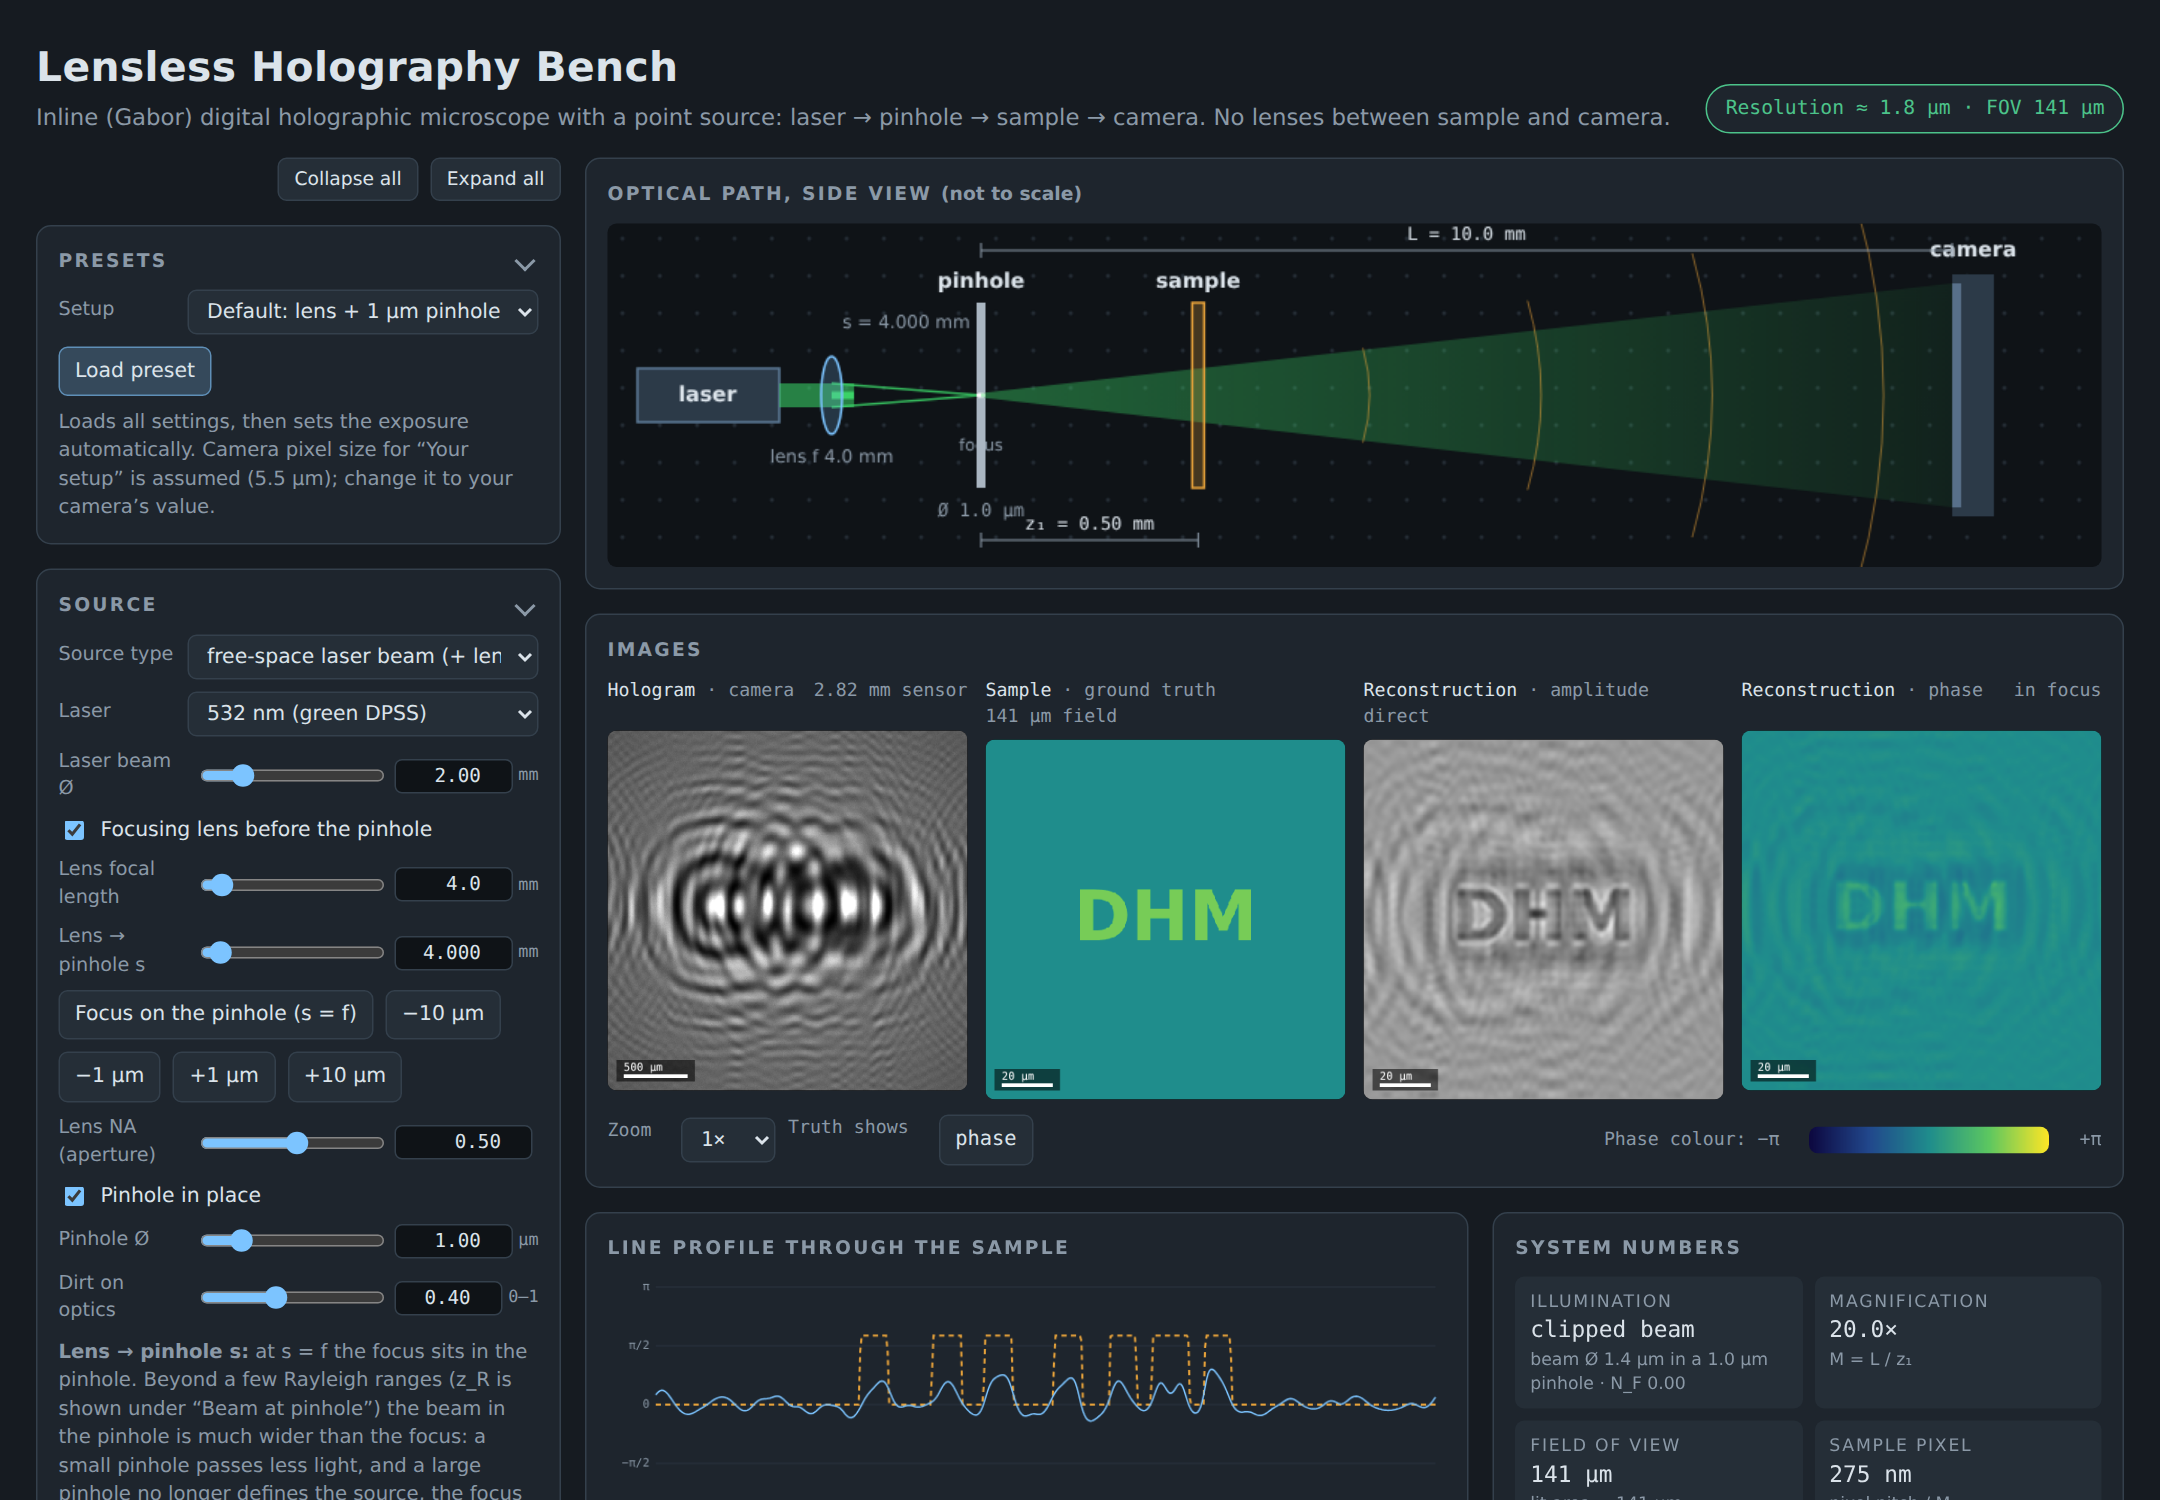
\includegraphics[width=\linewidth]{app.png}
\caption{The simulator with the default lens + pinhole setup.}
\end{figure}

\begin{thebibliography}{9}
\bibitem{Goodman} J.~W. Goodman, \emph{Introduction to Fourier Optics}, 3rd ed., Roberts \& Company (2005).
\bibitem{Paganin} D.~M. Paganin, \emph{Coherent X-Ray Optics}, Oxford University Press (2006): Fresnel scaling theorem.
\bibitem{Matsushima} K.~Matsushima and T.~Shimobaba, ``Band-limited angular spectrum method for numerical simulation of free-space propagation in far and near fields,'' Opt.\ Express \textbf{17}, 19662 (2009).
\bibitem{GS} R.~W. Gerchberg and W.~O. Saxton, ``A practical algorithm for the determination of phase from image and diffraction plane pictures,'' Optik \textbf{35}, 237 (1972).
\bibitem{Latychevskaia} T.~Latychevskaia and H.-W. Fink, ``Solution to the twin image problem in holography,'' Phys.\ Rev.\ Lett.\ \textbf{98}, 233901 (2007).
\bibitem{Evans} E.~Evans and Y.-C. Fung, ``Improved measurements of the erythrocyte geometry,'' Microvasc.\ Res.\ \textbf{4}, 335 (1972).
\bibitem{ChenLam} N.~Chen and E.~Y. Lam, ``Differentiable pixel-super-resolution lensless imaging,'' Opt.\ Lett.\ \textbf{50}(4), 1180--1183 (2025).
\end{thebibliography}
\end{document}
